\documentclass[twoside,twocolumn]{article}

\usepackage{blindtext} 
\usepackage{graphicx}
\usepackage[sc]{mathpazo} 
\usepackage[T1]{fontenc} 
\linespread{1.05} 
\usepackage{microtype} 

\usepackage[utf8]{inputenc} 


\usepackage[spanish,english]{babel} 



\usepackage[hmarginratio=1:1,top=32mm,columnsep=20pt]{geometry} 
\usepackage[hang, small,labelfont=bf,up,textfont=it,up]{caption} 
\usepackage{booktabs} 


\usepackage{lettrine} 


\usepackage{enumitem} 
\setlist[itemize]{noitemsep} 


\usepackage{abstract} 
\renewcommand{\abstractnamefont}{\normalfont\bfseries} 
\renewcommand{\abstracttextfont}{\normalfont\small\itshape} 


\usepackage{titlesec} 
\renewcommand\thesection{\Roman{section}} % 
\renewcommand\thesubsection{\roman{subsection}} 
\titleformat{\section}[block]{\large\scshape\centering}{\thesection.}{1em}{} 
\titleformat{\subsection}[block]{\large}{\thesubsection.}{1em}{} 


\usepackage{fancyhdr} 
\pagestyle{fancy} 
\fancyhead{} 
\fancyfoot{} 
\fancyhead[C]{Patrones de Diseño $\bullet$ Octubre 2020 $\bullet$ } 
\fancyfoot[RO,LE]{\thepage} 


\usepackage{titling} 


\usepackage{hyperref} 

\usepackage{listings}
\usepackage{xcolor}

\lstdefinestyle{sharpc}{language=[Sharp]C, frame=lr, rulecolor=\color{blue!80!black}}


%----------------------------------------------------------------------------------------
%	TILULOS
%----------------------------------------------------------------------------------------


\setlength{\droptitle}{-4\baselineskip} 

\pretitle{\begin{center}\Huge\bfseries} 
\posttitle{\end{center}} 
\title{Patrones de Diseño} 
\author{Percy Taquila Carazas, Katerin Merino Quispe, Abraham Lipa Calabilla,
\\Edwart Balcon Coahila, Lisbeth Espinoza Caso}
\date{\today} 
\renewcommand{\maketitlehookd}{

\selectlanguage{english}
\begin{abstract}
\noindent 
Design patterns provide a coded mechanism for describing problems and their solution in a way that allows the software engineering community to design knowledge for reuse.
A pattern describes a problem, indicates the context and allows the user to understand the environment in which the problem occurs, and lists a system of forces that indicate how the problem can be interpreted in context, and the way in which the problem is applied. solution.
The Abstract Factory pattern is usually implemented with manufacturing methods that are also generally called from within the Template Method.
\end{abstract}


\selectlanguage{spanish}
\begin{abstract}
\noindent 
Los patrones de diseño dan un mecanismo codificado para describir problemas y su solución en forma tal que permiten que la comunidad de ingeniería de software diseñe el conocimiento para que sea reutilizado.
Un patrón describe un problema, indica el contexto y permite que el usuario entienda el ambiente en el que sucede el problema, y enlista un sistema de fuerzas que indican cómo puede interpretarse el problema en su contexto, y el modo en el que se aplica la solución.
El patron Abstract Factory suele implementarse con metodos de fabricacion que tambien generalmente son llamados desde el interior de Template Method.
\end{abstract}

}

%----------------------------------------------------------------------------------------

\begin{document}

% Print the title
\maketitle

%----------------------------------------------------------------------------------------
%	INTRODUCCION
%----------------------------------------------------------------------------------------

\section{Introduccion}

\lettrine[nindent=0em,lines=3]{L}os patrones de diseño son muy interesantes para los programadores, ya que nos ofrecen soluciones a problemas comunes y cuotidianos a la hora de diseñar una aplicación. Existen infinidad de casos en que el problema sigue el mismo patrón, solo cambia el contexto; un patrón de diseño te propone una solución a este tipo de problemas.\\

La manera de utilizarlos depende de dos factores: comprender correctamente cuando se pueden usar y tenerlos presentes a la hora de diseñar. Lo primero se consigue habiéndolos estudiado y puesto en práctica en diferentes contextos. Lo segundo, que también incluye su dificultad, es la capacidad de encontrarse con un problema, y ser capaz de relacionarlo con un patrón de diseño que conozcas.[1]

Las características de un patrón son tres:

\begin{itemize}
\item Contexto: situación en la que se presenta el problema de diseño.
\item Problema: descripción del problema a resolver, y enumeración de las fuerzas a equilibrar (requisitos no funcionales como eficiencia, portabilidad, cambiabilidad, …).
\item Solución: conjunto de medidas que se han de tomar, como crear alguna clase, atributo o método, nuevos comportamientos entre clases, …
\end{itemize}


%----------------------------------------------------------------------------------------
%	Desarrollo
%----------------------------------------------------------------------------------------


\section{Desarrollo}


\subsection{Patrones de diseño estructurales}

Consisten en configurar la estructura de nuestra aplicación para cumplir con los principios SOLID, así como mejorar la usabilidad y la mantenibilidad del código. Podemos aplicar los muy conocidos métodos de:

\begin{itemize}
\item Herencia
\item Composición
\item Agregación
\end{itemize}

También debemos tener en cuenta que hay tres formas de definir estructuras de datos:

\begin{itemize}
\item Estáticamente
\item Generado por código
\item Dinámicamente
\end{itemize}

\subsubsection{Adaptadores}

Tal como el nombre lo dice, mediante este patrón de diseño, podemos adaptar la funcionalidad de una clase a través de una interfaz.[2]

Si tenemos una clase Punto y una clase Linea:
\lstset{breaklines=true,style=sharpc}
\begin{lstlisting}
public class Punto
{
    public int X, Y;
}
public class Linea
{
    public Punto Inicio, Fin;
}
\end{lstlisting}

Pensamos en una Figura como una colección de Líneas:
\lstset{breaklines=true,style=sharpc}
\begin{lstlisting}
public abstract class Figura : Collection<Linea> {}
\end{lstlisting}

Y creamos una clase Rectangulo a partir de la clase Figura (mediante herencia)
\lstset{breaklines=true,style=sharpc}
\begin{lstlisting}
public class Rectangulo : Figura
{
    public Rectangulo(int x, int y, int ancho, int alto)
    {
        // Codigo que agrega lineas a la coleccion
    }
}
\end{lstlisting}

Nos toparemos con un problema. En la interfaz que tenemos para pintar en pantalla tenemos un método que solo funciona con Puntos.
\lstset{style=sharpc}
\begin{lstlisting}
public static void PintarPunto(Punto p)
{
    // Codigo para pintar en las coordenadas X, Y de p
}
\end{lstlisting}

Para solucionar eso, tenemos los Adaptadores. Necesitamos que el adaptador "convierta" una Línea en una colección de Puntos para que puedan ser pintados con la interfaz.
\lstset{style=sharpc}
\begin{lstlisting}
public class AdaptadorLineaAPunto : Collection<Punto>
{
    public AdaptadorLineaAPunto(Linea linea) {
        // Codigo para agregar los puntos en el recorrido de las Lineas
    }
}
\end{lstlisting}

Finalmente, implementamos la solución de la siguiente forma.
\lstset{style=sharpc}
\begin{lstlisting}
private static void PintarPuntos()
{
    foreach (var linea in rectangulo)
    {
        var adaptador = new AdaptadorLineaAPunto(linea);
        adaptador.ForEach(PintarPunto);
    }  
}
\end{lstlisting}

Tomamos cada Linea en el Rectangulo, almacenamos en una variable una instancia del adaptador y pintamos cada Punto en el adaptador.


\subsection{Patrones de diseño de comportamiento}
Los patrones de comportamiento tienen que ver con algoritmos con la asignación de responsabilidades a objetos, describen no solo patrones de clases y objetos, sino también patrones de comunicación entre ellos. Los patrones de comportamiento basados en clases usan la herencia para distribuir el comportamiento entre clases.[3]

\smallskip
\textbf{2.1. Template method (Método plantilla)}
Consiste en definir un algoritmo como un esqueleto de operaciones y dejar los detalles para que sean implementados por las clases secundarias. La clase principal conserva la estructura y secuencia general del algoritmo.[3]

Es decir usa la herencia para la distribución del comportamiento. En el patrón del método plantilla,  un algoritmo particular se define en el método plantilla, pero los pasos exactos de este algoritmo se pueden definir en subclases. El método plantilla se implementa en una clase abstracta.

\smallskip
Ejemplo: Comida es una clase abstracta con un método de plantilla llamado imprimir () que define los pasos involucrados en una comida. Declaramos el método como final para que no se pueda anular. 

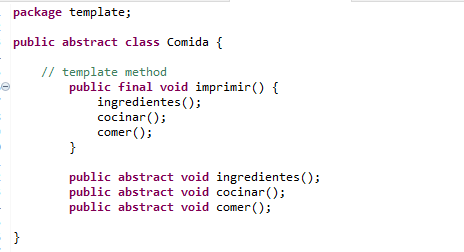
\includegraphics[width=8cm]{Imagenes/imagen}

La clase Hamburguesa extiende de Comida e implementa los tres métodos abstractos de Comida.

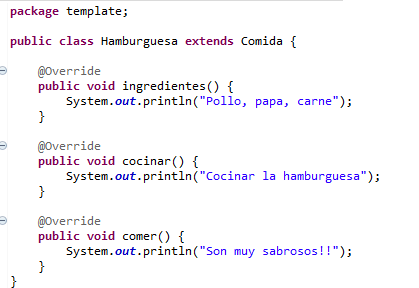
\includegraphics[width=8cm]{Imagenes/imagen2}

La clase Salchipapa extiende de Comida e implementa los tres métodos abstractos de Comida.

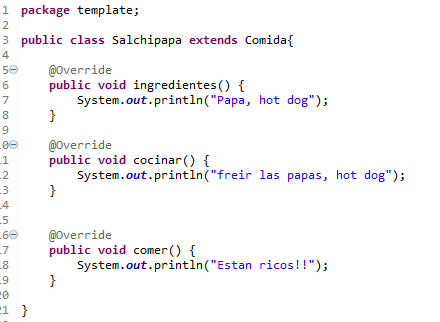
\includegraphics[width=8cm]{Imagenes/imagen3}

La clase Demo crea un objeto Hamburguesa y llama al metodo imprimir, luego se crea un objeto Salchipapa y llama a imprimir.

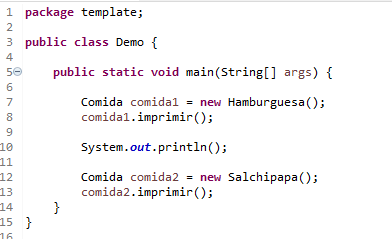
\includegraphics[width=8cm]{Imagenes/imagen4}

La salida de la consola de la ejecución.

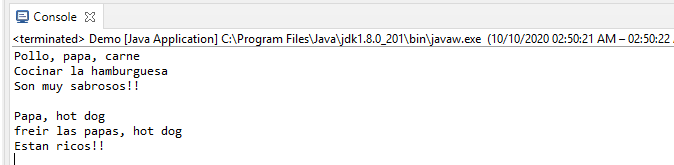
\includegraphics[width=8cm]{Imagenes/imagen5}


\subsection{Patrones de diseño creacionales}


Consisten en configurar la estructura de nuestra aplicación para cumplir con los principios SOLID, así como mejorar la usabilidad y la mantenibilidad del código. Podemos aplicar los muy conocidos métodos de:
Se ocupa de los mecanismos de creación de objetos, tratando de crear objetos de una manera adecuada a la situación.
En otras palabras, este patrón busca, de alguna manera “despreocupar” al sistema de cómo sus objetos son creados o compuestos.



\subsubsection{Singleton}


Este patrón involucra una sola clase que es responsable de crear un objeto mientras se asegura de que solo se cree un objeto, asegurar de que sólo posee una instancia y proporcionar un método de clase único que devuelva esta instancia.[4]




Si tenemos una clase Conexión, creamos un objeto, hacemos que el constructor sea privado para que no pueda ser instanciado y creamos un método para obtener la instancia únicamente por el mismo.
\lstset{breaklines=true,style=sharpc}
\begin{lstlisting}
public class clsConexion
{
    private static clsConexion cnxMySQL;

    private clsConexion() {
    }    

    public static clsConexion getInstancia() {
        if (cnxMySQL == null) {
            cnxMySQL = new clsConexion();
        }
        return cnxMySQL;
    }

    public Connection getConnection() {
        Connection Mysql = null;
        try {
            MysqlConnectionPool 
            DataSource ds = new MysqlConnectionPool DataSource();
            ds.setServerName("localhost");
            ds.setPort(3306);
            ds.setDatabaseName("db_modelo");
            Mysql = ds.getConnection("root", "");

        } catch (Exception ex) {
            JOptionPane.showMessageDialog(null, 'Error de conexion a la BD');
        }
        return Mysql;
    }
}
\end{lstlisting}


Y en las demás clases podemos instanciar sin necesidad del operador “new”:
\lstset{breaklines=true,style=sharpc}
\begin{lstlisting}
public class clsNegocioActividad implements clsInterfaceActividad {

    clsConexion c = clsConexion.getInstancia();

    @Override
    public void AgregarActividad(clsEntidadActividad Actividad) {
        try {
            Connection conexion = c.getConnection();
            CallableStatement cst = conexion.prepareCall("{call USP_Actividad_I(?,?,?)}");
            cst.setString("psemestre_id", Actividad.getSemestre_id());
            cst.setString("pcriterio_id", Actividad.getCriterio_id());
            cst.setString("pnombre", Actividad.getNombre());
            cst.execute();
        } catch (SQLException ex) {
            ex.printStackTrace();
        }
    }
}
\end{lstlisting}
\subsubsection{ Fábrica }


Sirve para construir una jerarquía de clases. Define una interfaz para crear un objeto, pero deja que sean las subclases quienes decidan qué clase instanciar. 


Primero creamos una clase interface
\lstset{breaklines=true,style=sharpc}
\begin{lstlisting}
public interface clsInterfaceConexion {

    void getConnection();
}
\end{lstlisting}


Luego declaramos clases que implementen la interface ya creada
\lstset{breaklines=true,style=sharpc}
\begin{lstlisting}
public class clsConexionMySQL implements clsInterfaceConexion {

    @Override
    public void getConnection() {
        Connection Mysql = null;
        try {
            MysqlConnectionPool DataSource ds = new MysqlConnectionPool DataSource();
            ds.setServerName("localhost");
            ds.setPort(3306);
            ds.setDatabaseName("db_modelo");
            Mysql = ds.getConnection("root", "");

        } catch (Exception ex) {
            JOptionPane.showMessageDialog(null, 'Error de conexion a la BD');
        }
    }
    
}
\end{lstlisting}



Creamos la clase fábrica para generar un objeto de una clase según la información dada
\lstset{breaklines=true,style=sharpc}
\begin{lstlisting}
public class ConexionFabrica {

    public clsInterfaceConexion getConnection(String motor) {
        if (motor == null) {
            return new clsConexionVacia();
        } else if (motor.equalsIgnoreCase("MySQL")) {
            return new clsConexionMySQL();
        } else if (motor.equalsIgnoreCase("Oracle")) {
            return new clsConexionOracle();
        }
        return new clsConexionVacia();
    }

}
\end{lstlisting}



Y por último usamos la clase fábrica para obtener el objeto de la clase que solicitamos pasando algún tipo de información
\lstset{breaklines=true,style=sharpc}
\begin{lstlisting}
public class Aplicacion {
    public static void main(String[] args) {

        ConexionFabrica fabrica = new ConexionFabrica();

        clsInterfaceConexion cx1 = fabrica.getConnection("MySQL");
        cx1.getConnection();

        clsInterfaceConexion cx2 = fabrica.getConnection("Oracle");
        cx2.getConnection();

    }
}
\end{lstlisting}



%----------------------------------------------------------------------------------------
%	Conclusiones
%----------------------------------------------------------------------------------------


\section{Conclusiones}

La conclusión es sencilla, si no usas patrones, deberías hacerlo. Los patrones ayudan a estandarizar el código, haciendo que el diseño sea más comprensible para otros programadores. Son muy buenas herramientas, y como programadores, siempre deberíamos usar las mejores herramientas a nuestro alcance

%----------------------------------------------------------------------------------------
%	Recomendaciones
%----------------------------------------------------------------------------------------

\section{Recomendaciones}


\begin{itemize}
\item Cuando se conoce el efecto colateral que conlleva el patrón de diseño y es viable la aparición de este efecto.
\item Suministrar alternativas de diseño para poder tener un software flexible y reutilizable.

\end{itemize}



%----------------------------------------------------------------------------------------
%	BIBLIOGRAFIA
%----------------------------------------------------------------------------------------

\selectlanguage{spanish}
\begin{thebibliography}{99} 

\bibitem[1]{}
\newblock Gamma, Erich; Helm, Richard; Johnson, Ralph; Vlissides, John(1995).Design Patterns: Elements of Reusable Object- Oriented Software. Reading,Massachusetts: Addison Wesley Longman, Inc.

\bibitem[2]{}
\newblock Nesteruk, D. (2019). Design Patterns in .NET: Reusable Approaches C\# in and F\# for Object-Oriented Software Design (1st ed.). Apress.

\bibitem[3]{}
\newblock Patrones de Diseño. Elementos de software orientado a objetos reutilizable. ERICH GAMMA. RICHARD HELM. RALPH JOHNSON. JOHN VLISSIDES.

\bibitem[4]{}
\newblock Patrones de diseño en Java: Los 23 modelos de diseño: descripción y solución ilustradas en UML 2 y Java Autor: Laurent Debrauwer

\end{thebibliography}


%----------------------------------------------------------------------------------------


\end{document}
